\subsection{Single-Chip mode y Expanded mode}
Los microprocesadores cuentan con una cantidad finita de accesos que, dependiendo de que tipo de pin sea, puede adoptar un carácter unidireccional o bidireccional. Para que la MCU tenga la posibilidad de interactuar con diferentes periféricos, es necesario que este tenga la habilidad de poder comunicarles cuando es que se los requiere. Esta conexión recibe el nombre de \textbf{chip-select}.

\begin{figure}[H]
	\centering
	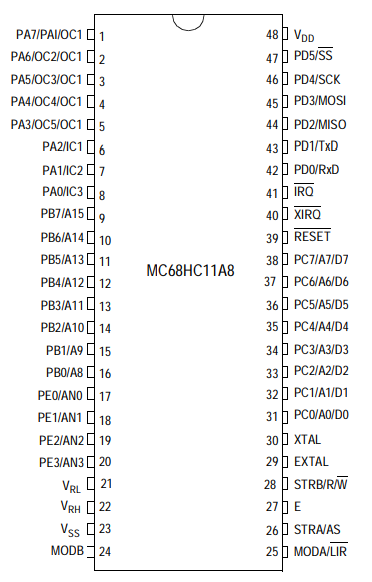
\includegraphics[scale=0.5]{ImagenesEjercicio3/MicroHC11}
	\caption{Microprocesador HC11}
	\label{fig:microhc11}
\end{figure}

El \textbf{HC11} posee un bus de datos de 8 bits y un puerto dedicado a indicar direcciones, el \textbf{address-bus}. Este puerto recibe el nombre de \textbf{Puerto B}. Este esta conformado por 8 bits. En single-chip-mode este puerto nos permitiría conectarnos con hasta 8 periféricos, es decir que nos provee con solo 8 lineas de chip-select.  Para poder acceder a memorias y chips adicionales se introduce el \textbf{expanded-mode}.
\begin{figure}[H]
	\centering
	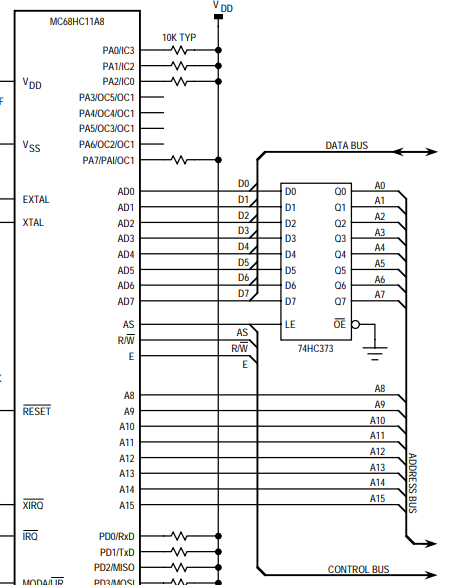
\includegraphics[scale=0.5]{ImagenesEjercicio3/MicroHC11ExpandedMode.PNG}
	\caption{Microprocesador HC11 en modo expandido}
	\label{fig:microhc11}
\end{figure}

 El modo expandido del \textbf{HC11} utiliza su bus de datos como un bus de address de manera temporal, este se encarga de escribir la parte baja de los nuevos 16 bits de address. Sin embargo, durante la comunicación con los periféricos, el bus de datos cumple la función de intercambiar datos o de dar instrucciones. Es por eso que se introduce un nuevo bloque a la salida del \textbf{Puerto C}, un bloque del tipo latch. Este se encarga de "recordar" la parte de baja que fue escrita por el bus de datos y dejarlo libre.
 Esto significa que ahora hemos conseguido duplicar la cantidad de lineas de chip-select disponibles consiguiendo 16 lineas. 
 Sin embargo es posible aumentar aún más el número de perifericos a los que se puede acceder si implementamos un \textit{decoder/demux} tal que el bus de address sea la entrada del mismo y el chip select sea su salida. La implementación más burda y directa de este decoder nos permitirá acceder a $2^{16} = 65536$ periféricos. No obstante, en la practica se utilizan diferentes circuitos de lógica digital que utilizan de forma más inteligente el bus de address. Además debemos considerar que si se utilizasen las 65536 lineas de chip-select antes mencionadas, el área que ocuparían sería excesivamente grande.
 
\subsection{Fanout}
Una vez resuelto el problema de \textbf{cómo} realizar la interconexión \textit{perifericos-cpu} cabe preguntarse el efecto que tendrán todas esas lineas conectadas a la cpu. Si se le demanda a la cpu por sobre su capacidad de \textbf{Fanout} se deben añadir buffers que añadirán retraso y por ende bajaran la velocidad máxima del sistema, pero sera capaces de soportar más cargas.
